\subsection{RM101变转速齿轮箱诊断案例}
\label{sec:rm101_case}

为验证本文提出的基于大语言模型智能体的自主信号处理框架在复杂工况下的诊断能力，本文进一步在 RM101 齿轮箱变转速数据集上开展案例研究。与前述 Ottawa 数据不同，RM101 同时包含转速变化与载荷变化，且故障类型既包括齿轮单一故障，也包括齿轮--轴承复合故障。因此，该数据集更适合检验自主规划图谱在复杂工况适应、物理语义保持以及多分支特征构造方面的综合能力。

\subsubsection{数据集与工况设置}

本案例使用 RM101 数据集中的 `Dataset\_id=101` 子集，并纳入全部 `12` 个工况域进行混合评估。具体协议为：先在原始长序列样本级别进行分层划分，再对每条长序列切分为长度为 `4096`、步长为 `4096` 的滑动窗口，以避免在窗口划分前混合样本而导致数据泄漏。最终得到训练、验证和测试原始样本分别为 `146/46/48` 条，对应窗口数为 `27448/8648/9024` 个。由于本实验采用的是 mixed-domain stratified split，因此结果反映的是多工况混合条件下的高精度诊断能力，而不是留一工况外推的泛化能力。

\subsubsection{通道定义与辅助输入设计}

RM101 数据包含 8 个同步测量通道，其中 `ch1` 为转速/键相信号，`ch2` 为转矩信号，`ch3$\sim$ch5` 为电机侧三向振动，`ch6$\sim$ch8` 为齿轮箱侧三向振动。本文并未将转速和转矩作为与振动完全等价的普通输入通道，而是将其设计为辅助侧输入：转速/键相信号主要服务于阶次跟踪与同步平均等速度感知算子，转矩信号则用于对高价值特征分支进行载荷归一化。由此，系统既能保持主诊断依据仍由振动信号提供，又能够在物理上利用工况侧信息对变转速、变载荷条件下的特征漂移进行修正。

\subsubsection{诊断图谱与主要结果}

表~\ref{tab:rm101_main_results} 给出了本案例的四组主结果，表~\ref{tab:rm101_dag_summary} 则进一步列出了对应图谱的结构复杂度。可以看到，随着 simulated planner complexity ladder 的提升，图谱深度、节点数以及算子多样性均明显增加。其中，`Gemini 2.5 Pro (simulated)` 对应的图谱最为丰富，其深度达到 `5`，节点数为 `52`，同时显式包含 `fft`、`psd`、`stft`、`patch`、`order\_track\_resample`、`tsa\_cycle\_average` 和 `torque\_normalize` 等关键物理算子。

\begin{table}[!htbp]
\centering
\caption{RM101 all-domain mixed 设定下的主结果对比}
\label{tab:rm101_main_results}
\resizebox{\textwidth}{!}{%
\begin{tabular}{lcccl}
\toprule
\textbf{方法} & \textbf{Test Accuracy} & \textbf{Test Macro-F1} & \textbf{Final Choice} & \textbf{备注} \\
\midrule
BigModel / GLM-4.7-FlashX（真实基线） & 0.8141 & 0.8229 & best\_single\_leaf & real baseline \\
Gemini 2.0 Flash（模拟，all-domain mixed） & 0.1539 & 0.1305 & weighted\_ensemble & simulated planner variant \\
Gemini 2.5 Flash（模拟，all-domain mixed） & 0.2585 & 0.2525 & best\_single\_leaf & simulated planner variant \\
Gemini 2.5 Pro（模拟，all-domain mixed） & \textbf{0.8865} & \textbf{0.8865} & best\_single\_leaf & richest simulated planner variant \\
\bottomrule
\end{tabular}%
}
\end{table}


\begin{table}[!htbp]
\centering
\caption{RM101 主图谱的结构复杂度对比}
\label{tab:rm101_dag_summary}
\resizebox{\textwidth}{!}{%
\begin{tabular}{lcccc}
\toprule
\textbf{方法} & \textbf{深度} & \textbf{节点数} & \textbf{边数} & \textbf{关键算子摘要} \\
\midrule
BigModel / GLM-4.7-FlashX & 3 & 20 & 12 & crest\_factor, kurtosis, psd, rms, spectral\_centroid \\
Gemini 2.0 Flash（模拟） & 3 & 20 & 12 & fft, psd, rms, kurtosis, crest\_factor, spectral\_centroid \\
Gemini 2.5 Flash（模拟） & 4 & 28 & 26 & coherence, order\_track\_resample, sideband\_ratio, torque\_normalize \\
Gemini 2.5 Pro（模拟） & \textbf{5} & \textbf{52} & \textbf{56} & fft, psd, stft, patch, order\_track\_resample, tsa\_cycle\_average, torque\_normalize \\
\bottomrule
\end{tabular}%
}
\end{table}


\begin{figure}[!htbp]
\centering
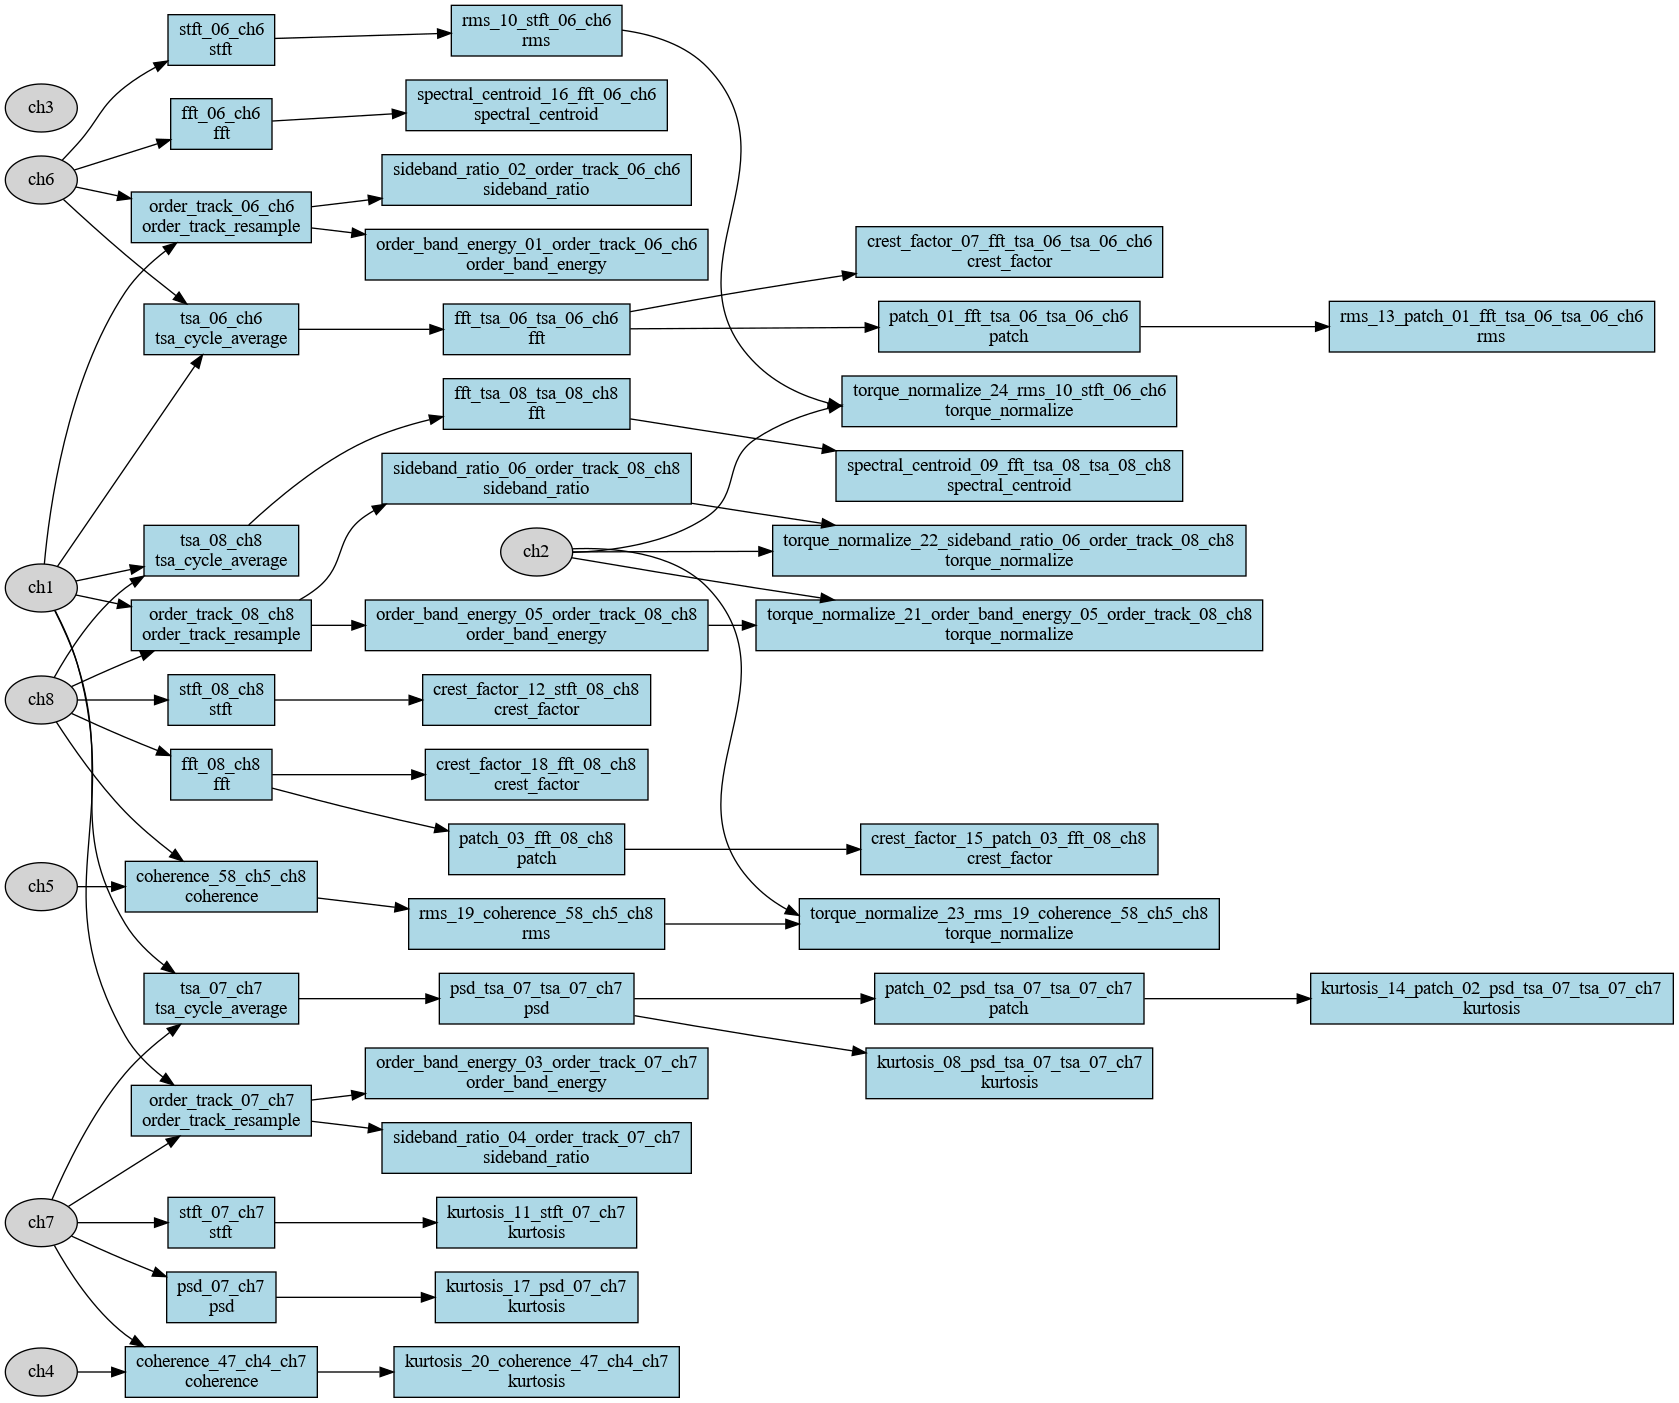
\includegraphics[width=0.92\textwidth]{figures/rm101_best_dag.png}
\caption{RM101 最优自主诊断图谱。该图谱来自 `Gemini 2.5 Pro (simulated, all-domain mixed)`，能够同时组织谱域、时频域、阶次域、跨通道关系与载荷归一化等多类诊断步骤。}
\label{fig:rm101_best_dag}
\end{figure}

从分类结果看，四组方案中最优结果来自 `Gemini 2.5 Pro (simulated, all-domain mixed)`，其测试集准确率与 Macro-F1 分别达到 `0.8865` 和 `0.8865`。相比之下，当前真实基线 `BigModel / GLM-4.7-FlashX` 的最佳单分支结果为 `Accuracy=0.8141`、`Macro-F1=0.8229`。这表明，在变转速与变载荷共同作用的复杂齿轮箱场景下，具备更丰富物理工具组合能力的自主图谱，能够显著提升最终诊断性能。

\subsubsection{最优诊断路径分析}

最优图谱中被自动选出的最佳终端叶子为 `torque\_normalize\_24\_rms\_10\_stft\_06\_ch6`，其对应的物理路径可概括为 `$stft \rightarrow rms \rightarrow torque\_normalize$`。从机理上看，这一路径首先利用短时傅里叶变换提取变转速条件下的局部时频结构，再利用均方根统计量对时频能量进行稳定压缩，最后借助转矩信号对载荷引起的幅值偏移进行归一化修正。由于 `ch6` 对应齿轮箱 X 向振动，该分支在实际意义上等价于：优先从齿轮箱主振动通道中提取时频能量模式，并结合载荷侧信息进行工况补偿。因此，该路径不仅具备较高的数值性能，也具有较强的工程可解释性。

\subsubsection{结果讨论}

值得注意的是，跨图谱 late fusion 的测试集 Macro-F1 为 `0.8299`，虽然优于部分较弱图谱，但仍未超过最佳单图谱的性能。这说明在本案例中，最优单图谱已经足够集中地捕获了主要故障判别信息，继续做跨图谱融合反而会引入性能较弱分支的干扰。综合来看，RM101 案例的核心结论可概括为：对于变转速齿轮箱诊断问题，仅依赖静态频谱统计难以充分应对复杂工况漂移；将时频分析、载荷归一化与速度感知算子纳入同一自主决策图中，能够显著提升最终诊断准确率与宏平均 F1。
